\chapter{Summary and Outlook}\label{sec:zusammenfassung}

\section{Main Results}

This work connects arithmetic properties of a quadratic sequence with
classical geometry and shows how a simple Diophantine structure gives
rise to a three-dimensional helix. The principal results are:

\begin{enumerate}
\item Quadratic sequence


\[
k(n) = \frac{1}{6}(2n^2 + 3n + 1)
\]


with integer values precisely for


\[
n \equiv 1,5 \pmod{6}.
\]



\item Alternating step sizes (minor/major steps) with explicit formula


\[
a_k = \frac{1}{2}\bigl[(12k+3) + (-1)^{k+1}(4k+1)\bigr], \qquad k \geq 1.
\]



\item Circle circumferences


\[
U_m = 24m - 5
\]


with constant difference


\[
\Delta R = \frac{12}{\pi}.
\]



\item Archimedean spiral


\[
r(\theta) = \frac{6}{\pi^2}\theta.
\]



\item Simplified parametrisation via $p$:


\[
r(p) = \frac{6}{\pi\sqrt{3}}\sqrt{p},
\qquad
\theta(p) = \frac{\pi}{\sqrt{3}}\sqrt{p}.
\]



\item Exact arc-length integral


\[
L = \int_{p_1}^{p_2}
\frac{1}{\pi}\sqrt{\frac{3}{p} + \pi^2}\, dp.
\]



\item Taylor approximation with high accuracy:


\[
L \approx (p_2 - p_1)
+ \frac{3}{2\pi^2}\ln\!\left(\frac{p_2}{p_1}\right)
+ \frac{9}{8\pi^4}\left(\frac{1}{p_1} - \frac{1}{p_2}\right).
\]



\item Conical helix with half-angle


\[
\alpha = \arctan\!\left(\frac{2}{\pi}\right)
\approx 32.48^\circ.
\]



\item Integer points on the helix:


\[
\theta_n = \frac{\pi}{3}n + \frac{\pi}{4}.
\]



\item All primes $p>3$ appear as discrete points on the helix.
This follows as a corollary from the fact that all primes $p>3$
satisfy the congruence condition $p\equiv1,5\pmod{6}$ by a classical
result of number theory, and the helix is constructed so as to contain
all indices from these congruence classes. The helix additionally
contains all composite numbers with $n\equiv1,5\pmod{6}$; the primes
form a distinguished subset therein.
\end{enumerate}

\section{Methodological Significance}

This work demonstrates that arithmetic structures can not only be visualised
but \emph{geometrically forced}. The connection between:

\begin{itemize}
\item Number theory (congruences, prime numbers),
\item Analysis (integrals, Taylor series),
\item Geometry (spirals, cones, helices),
\item Classical constants ($\pi$, $\zeta(2)$)
\end{itemize}

leads to a surprisingly coherent three-dimensional structure.

The helix follows necessarily from:



\[
\Delta n = 6,
\qquad
\Delta r = \frac{12}{\pi},
\qquad
r \sim \sqrt{p},
\qquad
\theta \sim \sqrt{p}.
\]



\begin{figure}[htbp]
  \centering
  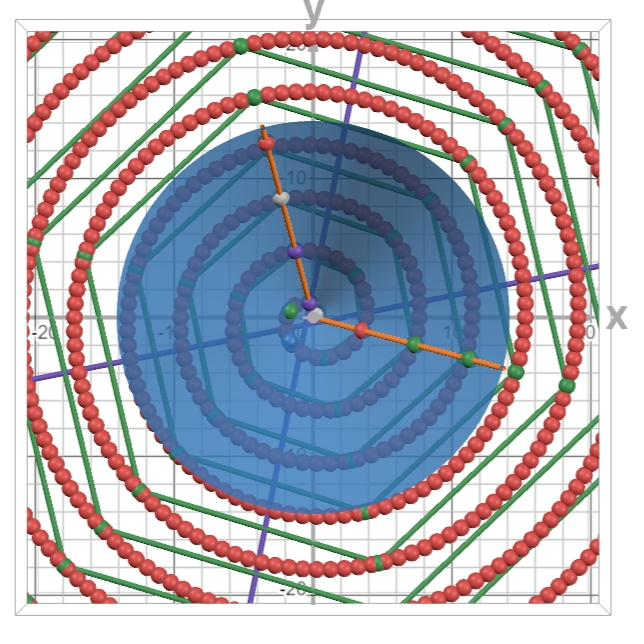
\includegraphics[width=0.72\textwidth]{bilder/spirale_topview}
  \caption{Top view of the conical helix (projection onto the $xy$-plane).
    The red spheres mark the equidistantly distributed points of the sequence
    on the spiral path. The green points (arranged hexagonally on six rays)
    show the function values $k(n)$ for all residue classes
    modulo~$6$; only the two rays with $n \equiv 1, 5 \pmod{6}$ yield
    integer values. The two diagonals run along these
    residue classes and make the $6$-periodicity of the arithmetic
    structure visually apparent. The blue disc shows the cone surface
    in projection; the spiral grows from inside to outside proportionally
    to $r \sim \theta$ (Archimedean).}
  \label{fig:spirale_topview}
\end{figure}

\section{Outlook}

The construction opens up several avenues for further investigation:

\begin{itemize}
\item \textbf{Prime gaps on the helix:}
  How do the distances between primes behave in the 3D model?

\item \textbf{Systematic comparison with the Ulam and Sacks spirals:}
  While the Ulam spiral~\cite{Stein1964} and the Sacks spiral~\cite{Sacks2003}
  are empirically motivated, the present construction possesses a closed-form
  derivation. A detailed comparison of the prime distributions
  across all three spiral types remains open.

\item \textbf{Generalisation to higher polynomial degrees:}
  Which geometries arise from cubic or quartic sequences?

\item \textbf{Modular interpretations:}
  Is there a connection to modular forms or lattice structures?

\item \textbf{Dynamical systems:}
  Can the helix be interpreted as the trajectory of a flow?

\item \textbf{Asymptotic analysis:}
  The exact 3D curvature (Theorem~\ref{thm:3d-curvature-torsion}) and torsion
  are now known; their finer asymptotic analysis, particularly at
  the prime points, remains open.
\end{itemize}

This work shows that even simple sequences such as


\[
k(n) = \frac{2n^2 + 3n + 1}{6}
\]


possess a remarkably rich geometric structure when consistently
transferred into three-dimensional space.
